% !TeX root = Protokoll.tex
\subsection{Amplitudenmodulation}
\begin{figure}[h!]
	\centering
	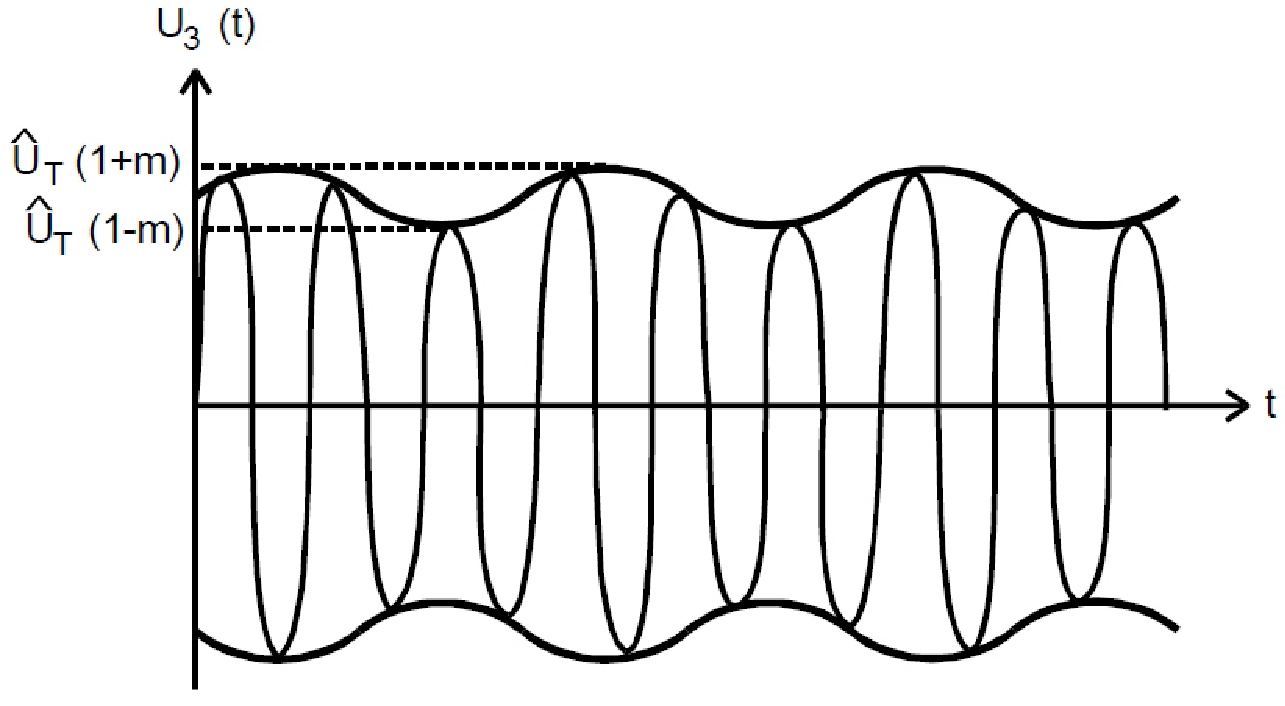
\includegraphics[width = 0.75\textwidth]{../Grafiken/Frequenzbaender.pdf}
	\caption{Beispiel für eine Amplitudenmodulierte Spannung.\label{fig:modulationsgrad_amplitude}\cite{V59}}
\end{figure}
In einer Schaltung ist eine hochfrequente Trägerspannung $U_T$, die geschrieben werden kann als
\begin{align}
	U_T(t)=\hat U_T\cos\omega_Tt.
\end{align}
Dabei ist $\hat U_T$ die Amplitude und $\omega_T$ die Kreisfrequenz.
Diese wird mithilfe einer Modulationsspannung $U_M$ modelliert, diese wird beschrieben durch
\begin{align}
	U_M(t)=\hat U_M\cos\omega_Mt,
\end{align}
mit der Amplitude $\hat U_M$ und der Kreisfrequenz $\omega_M$.
Die Spannung $U_3$die aus der Modulation entsteht kann geschrieben werden als
\begin{align}
	U_3(t)=\hat U_t\left(1+m\cos\omega_Mt\right)\cos \omega_Tt
\end{align}
mit dem Modulationsgrad $m$, der definiert ist als 
\begin{align}
	m = \gamma \hat U_M
\end{align}
mit der Proportionalitätskonstante $\gamma$ mit der Dimension $\frac{1}{V}$.
Das $m$ liegt zwischen 0 und 1.
Die Spannung $U_3$ kann umgeschrieben werden in
\begin{align}
	U_3(t)=\hat U_T\left[\cos\omega_Tt+\frac{1}{2}m\cos\left(\omega_T+\omega_M\right)t+\frac{1}{2}\cos\left(\omega_t-\omega_M\right)t\right]
\end{align}
Daraus lässt sich das Frequenzspektrum ablesen, dieses ist in \cref{fig:Frequenzspektrum} dargestellt.
Der einfachste Amplitudenmodulator ist die Diode, weil sie das eine nicht Lineare Kennlinie besitzt.
Durch das anlegen zweier Spannungen, ensteht das Produkt zweier Spannungen. 
\begin{align}
	I(U_T+U_M)=a_0+a_1(U_T+U_M)+a_2\left(U_T^2+U_M 2\right)+2a_2U_MU_T
\end{align}
Allerdings treten in der Reihenentwicklung der Diode auch unerwünschte Terme auf, wie zum Beispiel $U_T$, $U_M^2$ und $U_T^2$.

\begin{figure}
	\centering
	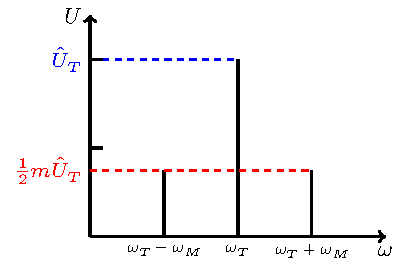
\includegraphics[width =\textwidth/2]{../Grafiken/tikz/tikz-Frequenzspektrum.pdf}
	\caption{Das Frequenzspektrum zu der Amplitudenmodulation.\label{fig:Frequenzspektrum} }
\end{figure}
\newpage
\begin{figure}
	\centering
	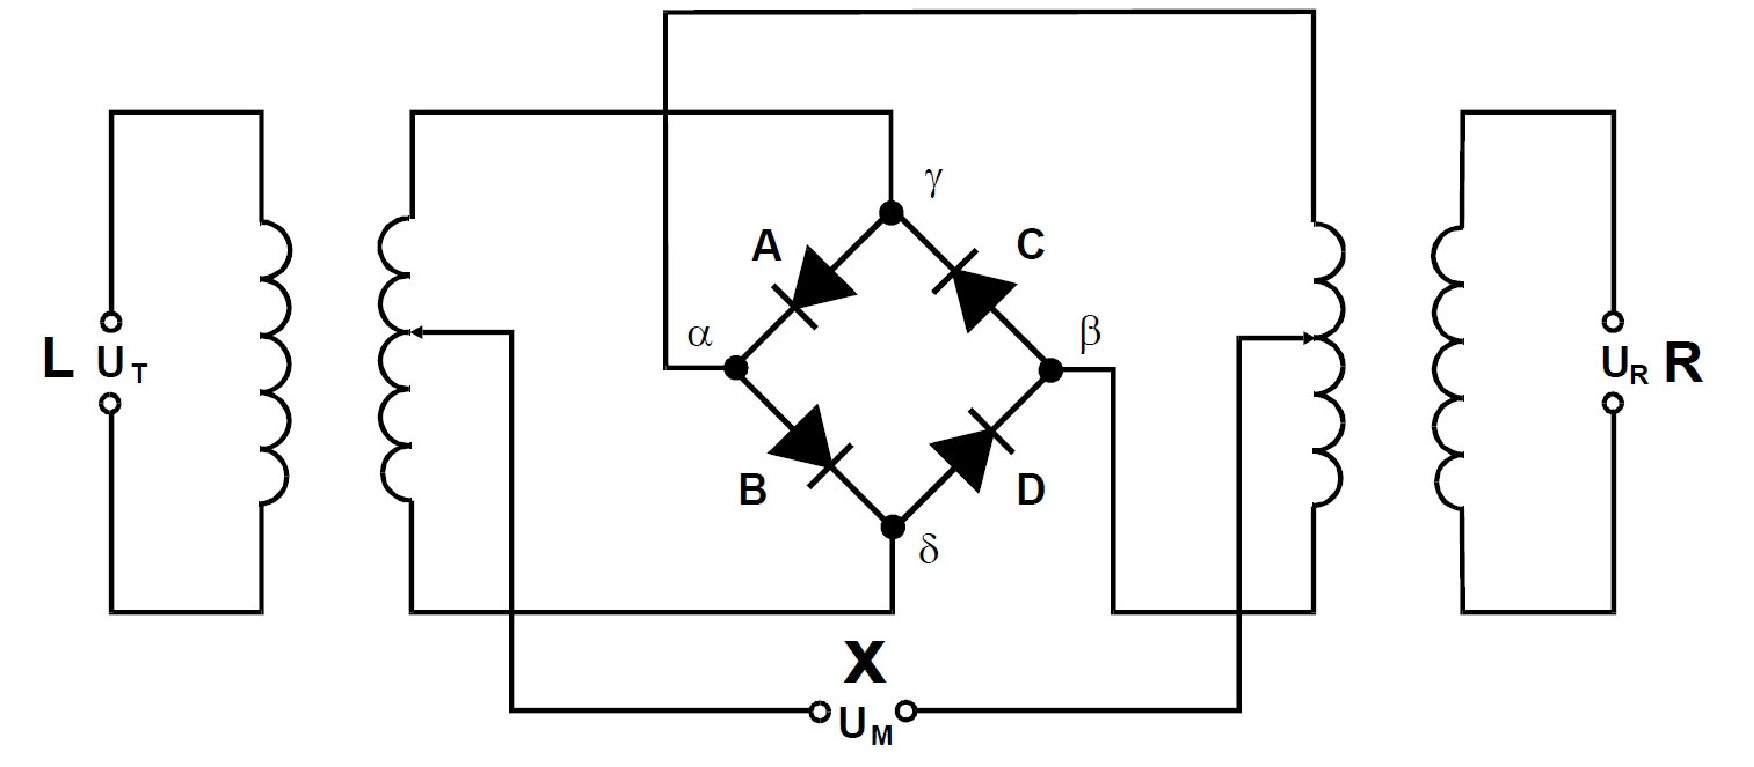
\includegraphics[width = 0.75\textwidth]{../Grafiken/Ringmodulator.pdf}
	\caption{Eine Skizze eines Ringmodulators.\cite{V59}\label{fig:Ringmodulator}}
\end{figure}
Um dies zu umgehen wird ein Ringmodulator verwendet, die besteht aus 4 im Ring angeordneten Dioden, wie in \cref{fig:Ringmodulator} dargestellt.
Am Punkt L liegt die Trägerspannung an und am Punkt X die Modulationsspannung.
Daraus folgt für die modulierte Spannung am Punkt R
\begin{align}
	U_R(t)=\Gamma\cdot \hat U_M(t) \cdot\hat U_T(t),
\end{align}
wobei $\Gamma$ eine Proportionalitätkonstante ist. Unter Berücksichtigung, dass die Spannung $U_M$ und $U_T$ um eine Phase $\phi$ verschieden Schwingen können, folgt
\begin{align}
	U_R(t)=\Gamma\cdot \frac{\hat U_T\cdot\hat U_M}{2}\left[ \left(\cos\left(\omega_T+\omega_M\right)t+\phi\right) +\cos\left(\left(\omega_T-\omega_M\right)t-\phi\right) \right].
	\label{eq:amplituden_moduliert_ohne_traeger}
\end{align}
Daraus lässt sich erkennen das nur noch die beiden Äußeren Frequenzen auftreten.

\newpage
\subsection{Frequenzmodulation}
\begin{figure}[h!]
	\centering
	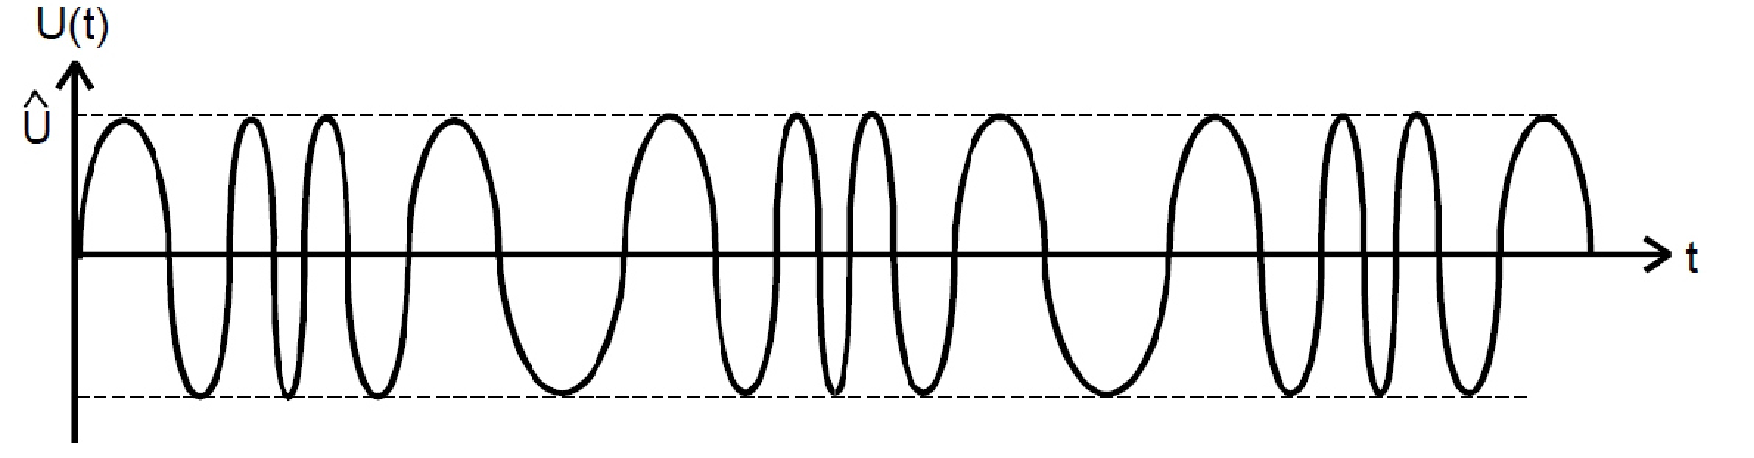
\includegraphics[width = \textwidth]{../Grafiken/Frequenzmodulation.pdf}
	\caption{Darstellung der Änderung einer Frequenzmodulierten Spannung gegen die Zeit.\cite{V59}\label{fig:Frequenzmodulation}}
\end{figure}
Bei der frequenzmodulierten Spannung, ändert sich die Phase beziehungsweise die Frequenz periodisch, wie in \cref{fig:Frequenzmodulation} dargestellt.
Die Spannung einer solcher modulierten Schwingung kann dargestellt werden durch
\begin{align}
	U(t)=\hat U \sin\left(\omega_Tt+m\frac{\omega_T}{\omega_M}\cos\omega_Mt\right)
\end{align}
Daraus lässt sich die momentan Frequenz $f$ bestimmen, durch Ableitung des Arguments vom Sinus.
\begin{align}
	f(t)=\frac{\omega_T}{2\pi}\left(1-m\sin\omega_Mt\right)
\end{align}
Daraus lässt sich der Frequenzhub ablesen als
\begin{align}
	\Delta \omega = m\frac{\omega_T}{2\pi}
\end{align}
\begin{figure}
	\centering
	%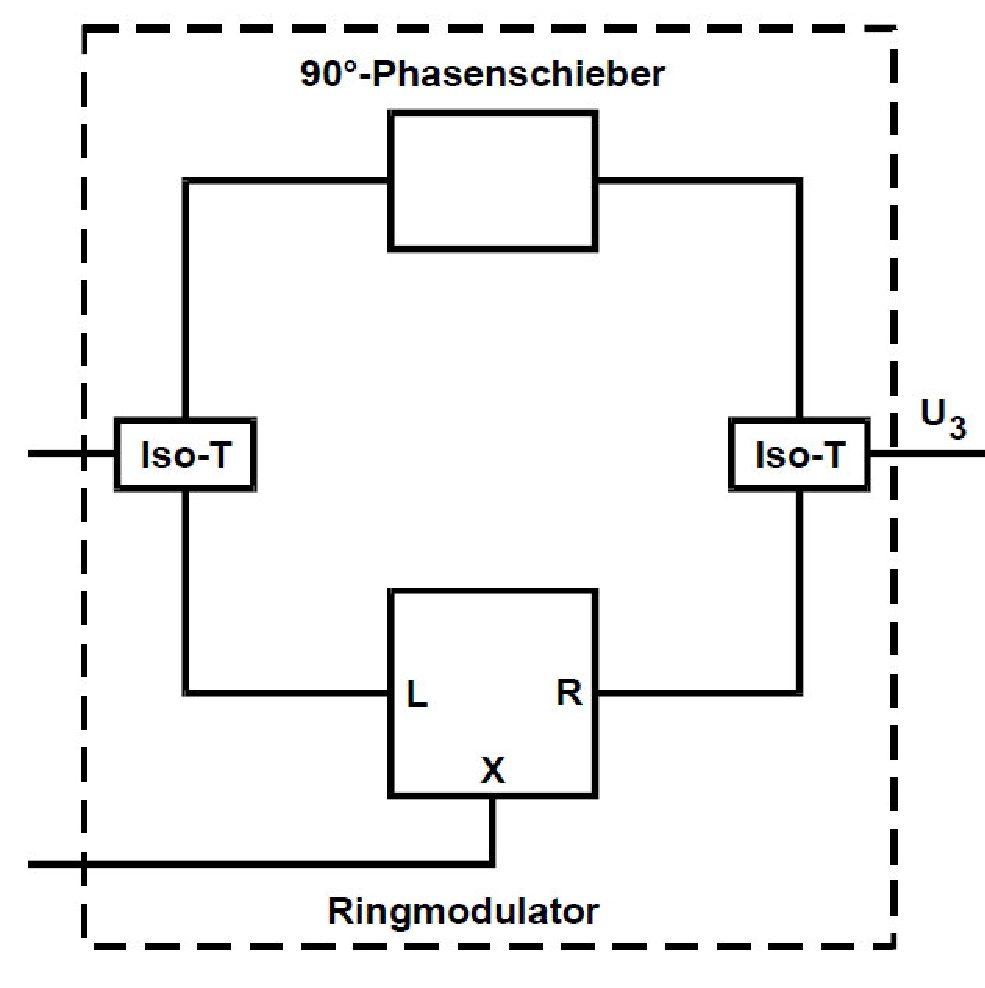
\includegraphics[width =0.75\textwidth/2]{../Grafiken/Schaltung_Frequenzmodulation.pdf}
\begin{tikzpicture}
			\node [draw=white, anchor=south west] (label) at (0,0) {
				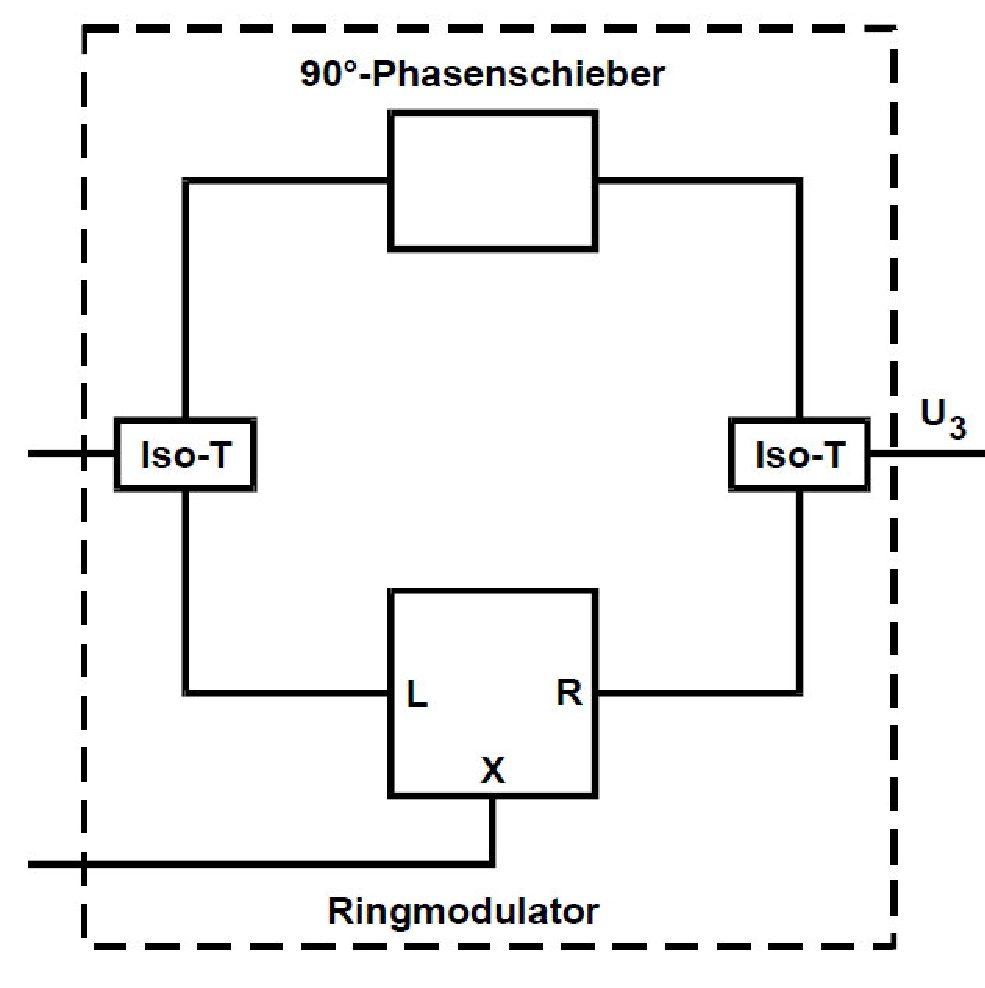
\includegraphics[width=\textwidth/2]{../Grafiken/Schaltung_Frequenzmodulation}};
			\node at (0.9 , 1.4) [left]{$\boldsymbol{U_M}$};
			\node at (0.9 , 4.75) [left]{$\boldsymbol{U_T}$};
						
			\fill[white] (7.9,4.92) circle(0.4);
			\node at (8,4.75){$\boldsymbol U_3$};
		\end{tikzpicture}
	\caption{Schaltung für eine Frequenzmodulation.\cite{V59}\label{fig:Schaltung_Frequenzmodlation}}
\end{figure}
Eine Schaltung für eine Frequenzmodulation ist in \cref{fig:Schaltung_Frequenzmodlation} dargestellt.
Dabei wird ein Ringmodulator verwendet, der nur noch Frequenzen $\omega_T+\omega_M$ und $\omega_T-\omega_M$ zulässt.
Zusätzlich wird ein $90^\circ$-Phasenschifter verwendet, mit dem die phasenverschobene Trägerspannung auf die Spannung der modellierten auf addiert wird.
Daraus entsteht eine frequenzmodelierte Schwingung

\newpage
\subsection{Demodulation von Schwingungen}
Eine Möglichkeit amplitudenmodellierte Schwingungen zu demodullieren ist der Ringmodulator.
Wenn am Eingang R eine modellierte Schwingung mit den Frequenzen $\omega_T+\omega_M $ und $\omega_T-\omega_M$ anliegt und an Eingang L eine Spannung mit der Kreisfrequenz $\omega_T$, dann liegt am Ausgang X eine Spannung mit den Frequenzen $2\omega_M$, $\omega_T+\omega_M $ und $2\omega_T+\omega_M $ an.
Mithilfe eines Tiefpasses kann die Frequenz $\omega_M$ heraus gefiltert werde. Diese Methode kann nur angewendet werden, wenn die Frequenz der Trägerspannung zur Verfügung steht.\\
Dieses Problem besteht nicht, wenn mithilfe einer Diode und eines Tiefpasses demodelliert wird.
Allerdings ist aufgrund der Kennlinie der Diode eine Verzerrung der Modulationsspannung zu erwarten.
Dies kann verhindert werden, indem eine Gegentaktschaltung verwendet wird.\\
Die Demudulation einer frequenzmodellierten Schwingung, geschieht mithilfe eines LC-Schwingkreises. Dafür wird die Resonanzfrequenz des Schwingkreises so eingestellt, so dass die Trägerfrequenz $\omega_T$ auf der Steilen Flanke der Resonanzkurve liegt. Dieses Verfahren macht aus der frequenzmodellierten eine Amplitudenmodellierte Spannung.
\newpage
